\documentclass[12pt,a4paper]{article}
\usepackage[utf8]{inputenc}
\usepackage[russian]{babel}
\usepackage[left=2.00cm, right=2.00cm, top=2.00cm, bottom=2.00cm]{geometry}
\linespread{1.25}
\usepackage{setspace}
\usepackage{indentfirst}
\setlength{\parindent}{1.25cm}
\let\paragraph\ignorespaces
\usepackage{tabularx}
\usepackage{multirow}
\usepackage{graphicx}



\begin{document}
	
\begin{titlepage}
	
\begin{center}
	\large Университет ИТМО\\[5cm]
	\LARGE Практическая работа №2\\
	\normalsize по дисциплине <<Визуализация и моделирование>>\\[5cm]
\end{center}
\begin{flushright}
		\begin{minipage}{0.6\textwidth}
		\begin{flushleft}
			\large
			\singlespacing 
			\textbf{Автор:} Костылев Иван Михайлович\\
			\textbf{Поток:} 1.1\\
			\textbf{Группа:} K3240\\
			\textbf{Факультет:} ИКТ\\
			\textbf{Преподаватель:} Чернышева А.В.
		\end{flushleft}
	\end{minipage}
\end{flushright}

\vfill

\begin{center}
	{\large Санкт-Петербург, \the\year{ г.}}
\end{center}
 
\end{titlepage}
\normalsize


\large \textbf{Описание датасета}

\normalsize
	Датасет состоит из данных о студентах, их родителей и оценок, полученных ими по различным предметам. \\

Всего записей: 1000 \\


\large \textbf{Формальное описание}

\begin{tabular}{ | p{100pt} | p{100pt} | p{100pt} | p{40pt} | p{60pt} |}
\hline
Столбец & Описание & Значения & Формат & Шкала  \\ \hline
gender & пол студента & male / female & текст & Качеств номинальная \\ \hline
race/ethnicity & расовая классификация & group A / group B / group C / group D & текст & Качеств номинальная  \\ \hline
parental level of education & уровень образования родителей & collegue / school / bachelor's degree / others  & текст & Качеств номинальная  \\ \hline
lunch & оплата обеда & standart / free/reduced & текст & Качеств номинальная  \\ \hline
test preparation & подготовка к тесту & none / completed & текст & Качеств номинальная  \\ \hline
math score & оценка по математике & 0..100 & целое число & Колич относительная  \\ \hline
reading score & оценка по чтению & 0..100 & целое число & Колич относительная  \\ \hline
writting score & оценка по письму & 0..100 & целое число & Колич относительная  \\ \hline
\end{tabular}
\\


\newpage
\large \textbf{Описательная статистика}

\textbf{1. Соотношение студентов мужчин и женщин}\\
Фрагмент кода, запроса:
\begin{verbatim}
male_df = df.loc[df[GENDER] == "male"]
m_num = male_df.shape[0]
female_df = df.loc[df[GENDER] == "female"]
f_num = female_df.shape[0]

gender_pie = pd.DataFrame({"": [m_num, f_num]},
                        index=["Males", "Females"])
gender_pie.plot.pie(y="",
                    colors=["c", "m"],
                    autopct="%.1f",
                    fontsize=10,
                    figsize=(5, 5))
\end{verbatim}


График: \\

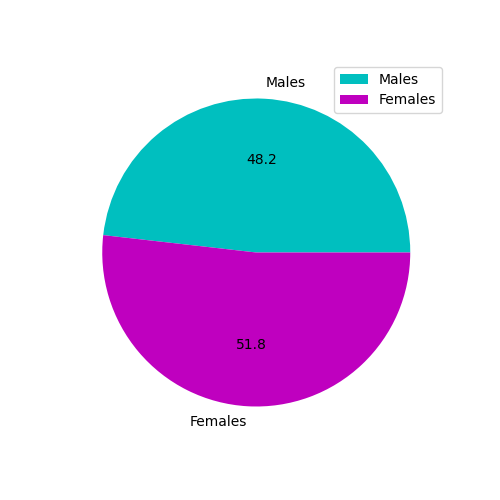
\includegraphics{male_female_1}

\large \textbf{Вывод:} можно считать равным количество студентов мужчин и женщин\\

\textit{Для решения следующих вопросов объявим для простоты константные переменные - названия полей}

\begin{verbatim}
READING = "reading score"
WRITING = "writing score"
MATH = "math score"
GENDER = "gender"
PLE = "parental level of education"
ETGROUP = "race/ethnicity"
PREPAR = "test preparation course"
\end{verbatim}

\textbf{Следующие вопросы связаны между собой:}

\textbf{2. Статистика по набранным баллам}

\textbf{3. Соотношение средних баллов к баллам по чтению}

\textbf{4. Соотношение средних баллов к баллам по письму}

\textbf{5. Соотношение средних баллов к баллам по математике}

Фрагмент кода, запроса:
\textit{Следующий код оказался слишком объемным, его можно посмотреть в исходном коде}


\large \textbf{График (2):} на рисунке по оси абсцисс - баллы от 0 до 100, а по оси ординат - количество человек, которые получили данный балл\\

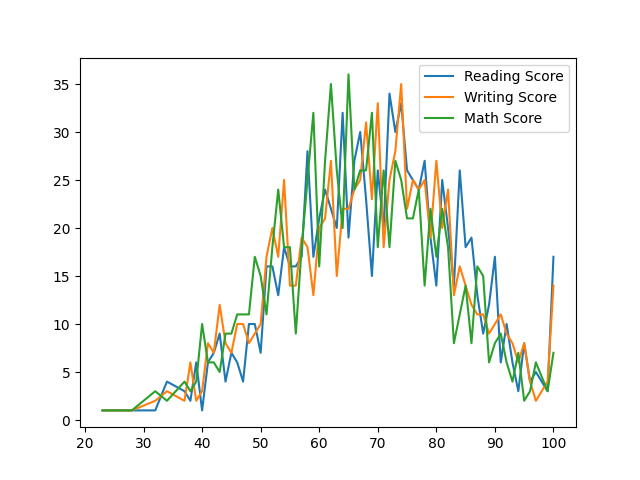
\includegraphics{all_scores}

\large \textbf{Вывод (2):} распределение по баллам примерно соответствует нормальному распределению. На данном графике не видно преобладание какого-либо предмета над другим. Для определения наиболее "успешного" (где средний балл выше) построить следующие графики:\\

\large \textbf{График (3):} средние оценки и оценки по чтению. На рисунке также по оси абсцисс - баллы от 0 до 100, а по оси ординат - количество человек, которые получили данный балл\\
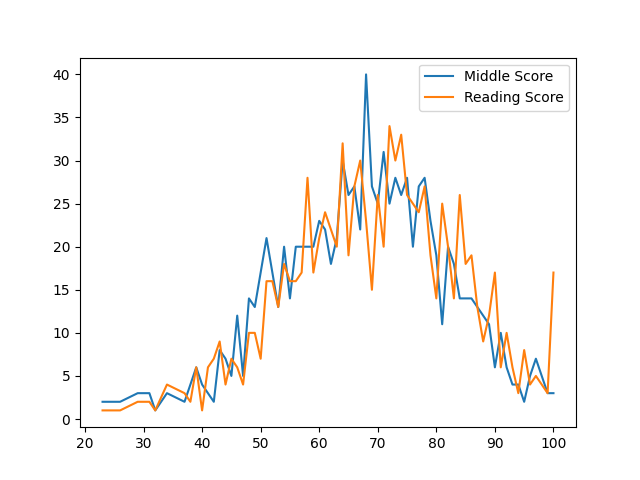
\includegraphics{middle_reading_score} 

\large \textbf{График (4):} средние оценки и оценки по письму\\
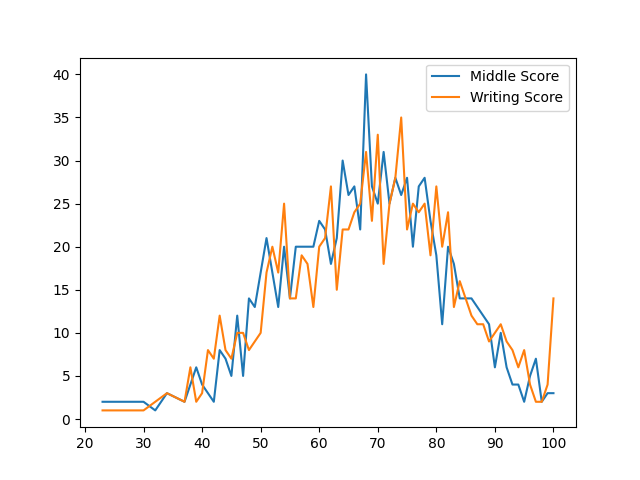
\includegraphics{middle_writing_score} 

\large \textbf{График (5):} средние оценки и оценки по математике\\
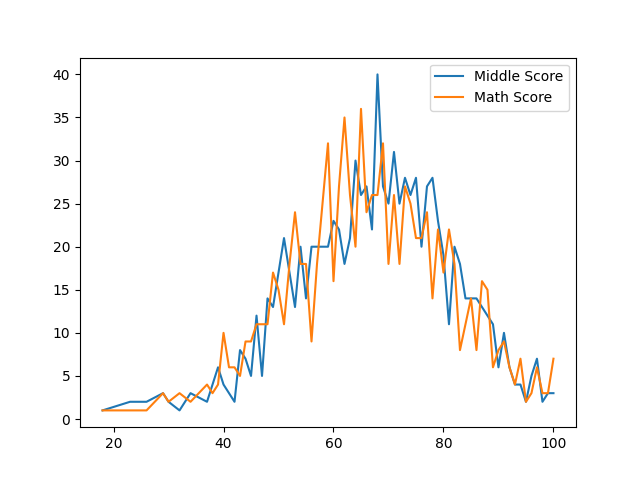
\includegraphics{middle_math_score} 

\large \textbf{Вывод (3-5):} из графика (5) видно, что баллы по математике ниже средних по всем предметам, так как график при баллах > 70 лежит ниже графика средних баллов. \textit{Можно построить гипотезу, что по математике средний балл ниже.}
В то же самое время из графика (3) видно, что здесь максимальное количество тех, кто получил 100 баллов, а также максимальная точка смещена вправо, что позволяет 
\textit{построить гипотезу, что по чтению средний балл самый высокий.}

Проверим далее наши предположения\\

\textbf{6. По какому предмету баллы, в среднем, выше?}

Фрагмент кода, запроса:
\begin{verbatim}
middle_scores = [middle_reading, middle_math, middle_writing]
subjects = ["Reading", "Math", "Writing"]

middles_df = pd.DataFrame({"subject": subjects, "middle score": middle_scores})
middles_df.plot.barh(x="subject", y="middle score", figsize=(12, 5))
\end{verbatim}

\textbf{График (6):}\\
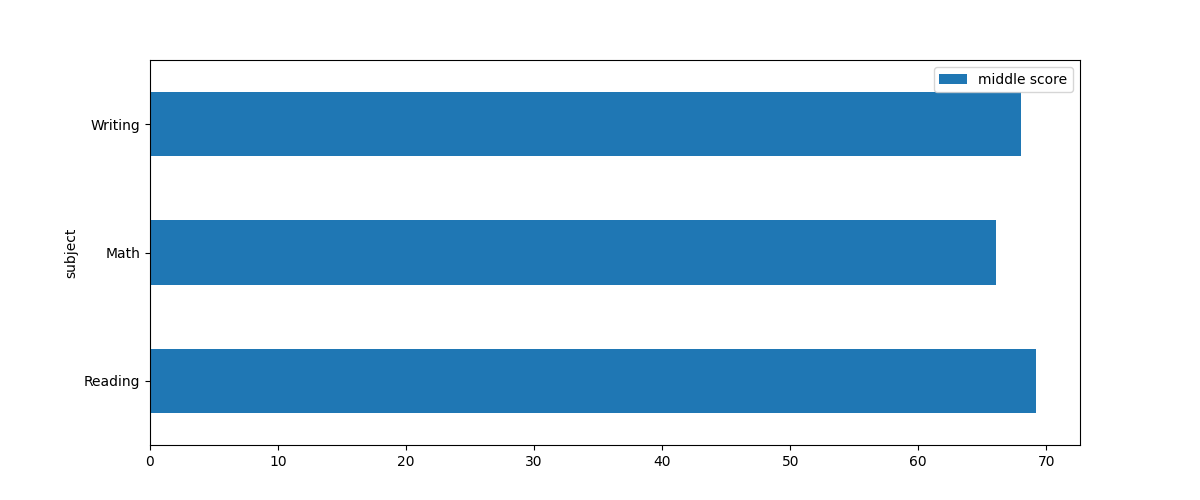
\includegraphics[scale=0.5]{middle_score_compare.png}

\large \textbf{Вывод:} гипотезы о том, что оценки по чтению в среднем выше, чем по остальным. Самые низкие получились по математике.


\textbf{7. Каково соотношение между этническими группами студентов?}

Фрагмент кода, запроса:
\begin{verbatim}
col = ETGROUP
groups_data = {name: df[col].to_list().count(name) for name in df[col].unique()}
groups_list = []
nums = []

for group, num in groups_data.items():
    groups_list.append(group)
    nums.append(num)

group_df = pd.DataFrame({"": nums}, index=groups_list)

group_df.plot.pie(y="",
                autopct="%.1f",
                fontsize=10,
                figsize=(12, 12))
\end{verbatim}
\textbf{График (7):}\\
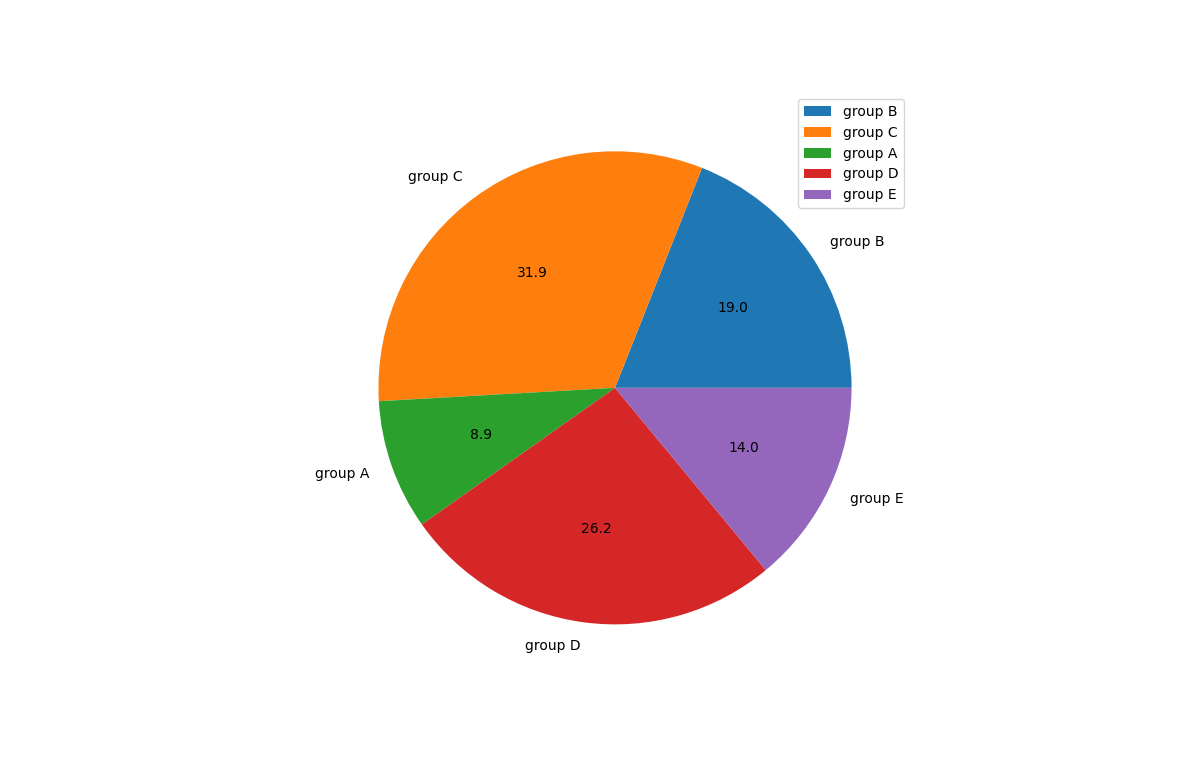
\includegraphics[scale=0.7]{race.png} 

\large \textbf{Вывод:} нельзя выделить какое-либо серьезное преобладание какой-либо группы (более 50 процентов). Самая распространенная группа, которая включена в статистику - группа D, самая менее распространенная - группа А.

\textbf{8. Как много студентов прошло подготовительный курс?}
\textbf{9. Существенна ли помощь подготовки?}


Фрагмент кода, запроса:
\begin{verbatim}
col = PREPAR
preparation_data = {name: df[col].to_list().count(name) for name in df[col].unique()}

preparations = []
nums = []

for prep, num in preparation_data.items():
    preparations.append(prep)
    nums.append(num)


prep_df = pd.DataFrame({"": nums}, index=preparations)

prep_df.plot.pie(y="",
                autopct="%.1f",
                fontsize=10,
                figsize=(12, 12))

\end{verbatim}
\textbf{График (8):}\\
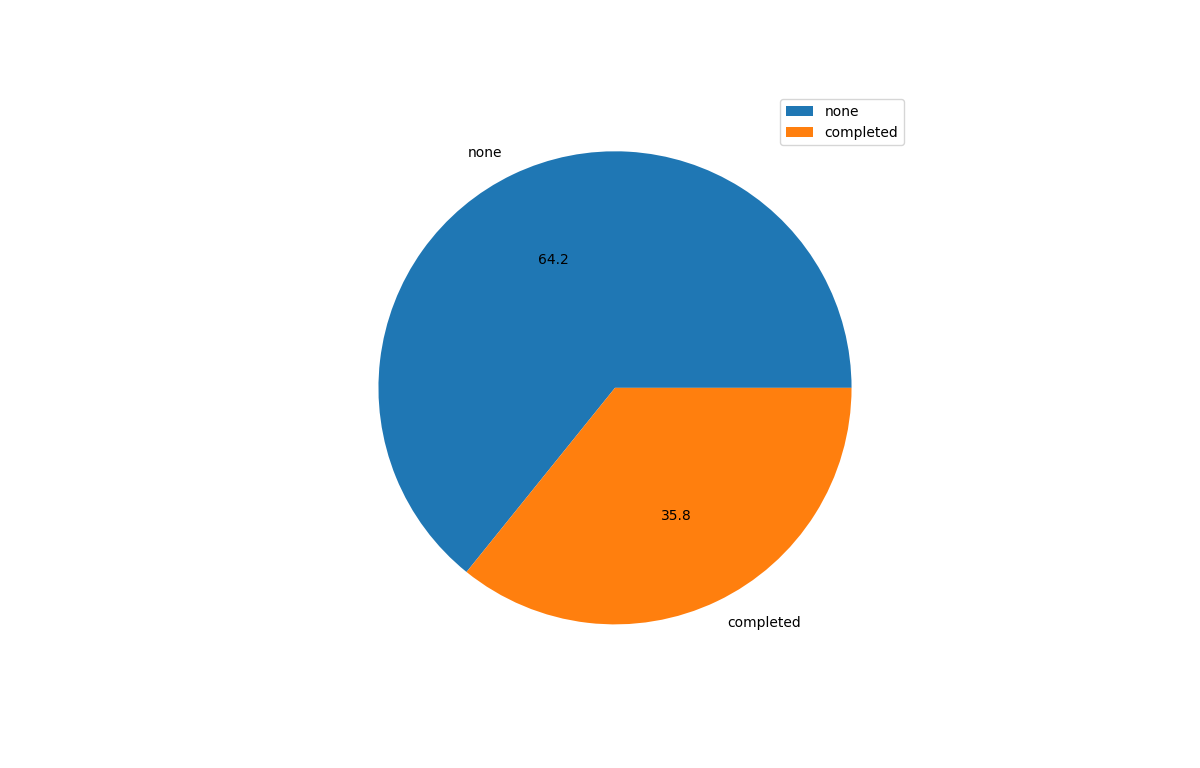
\includegraphics[scale=0.7]{preparation.png} 

\large \textbf{Вывод:} преобладают студенты, которые не проходили подготовительный курс. Посмотрим, выше ли баллы у студентов, которые его прошли\\

\textit{Следующий код оказался слишком объемным, его можно посмотреть в исходном коде}


\textbf{Получаем следующие графики (9):} здесь значения по оси y - доля людей от общего числа подготовившихся / не подготовившихся \\
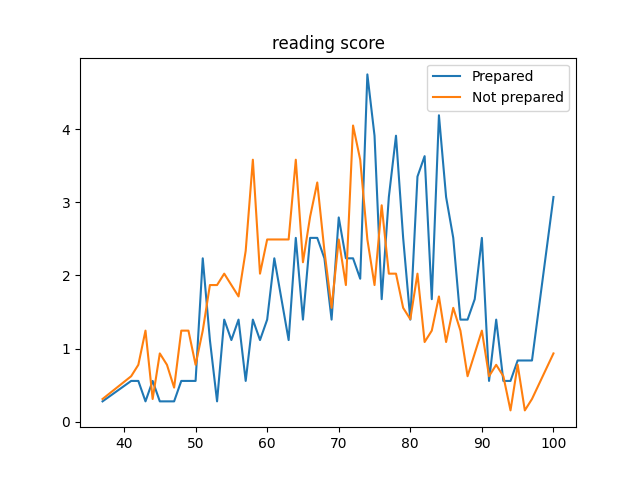
\includegraphics[scale=1]{prep_writing_score.png} 

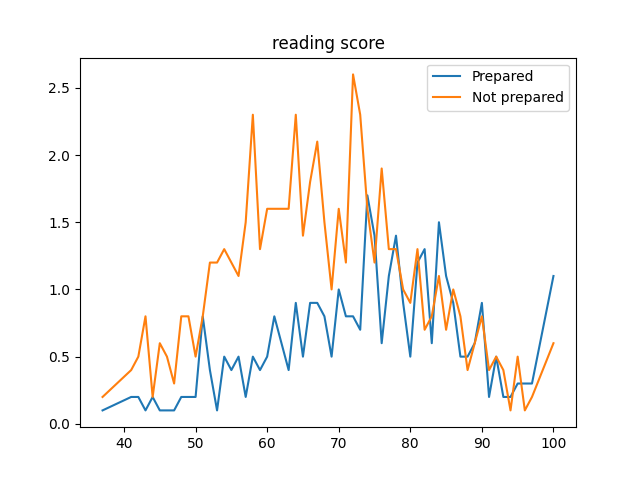
\includegraphics[scale=1]{prep_reading_score.png} 

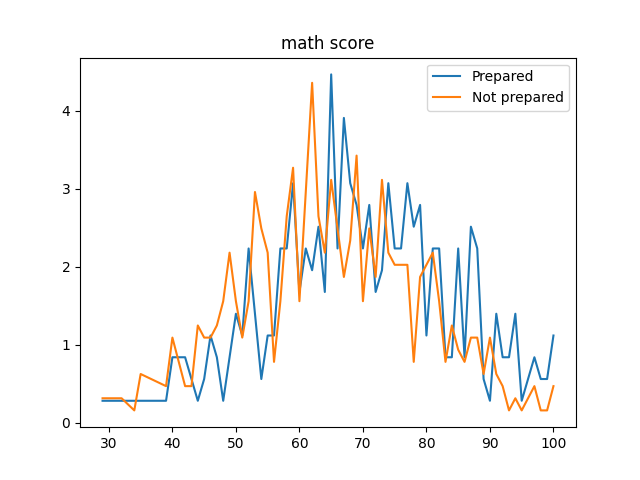
\includegraphics[scale=1]{prep_math_score.png}


\large \textbf{Вывод (9):} Ярче всего видно на графике чтения, что доля студентов, которые проходили курс, имеют более высокие баллы.
 
 
\textbf{10. Соотношение студентов мужчин и женщин}\\
Фрагмент кода, запроса:
\begin{verbatim}
or edu, num in par_edu_data.items():
        labels.append(edu)
        nums.append(num)

    par_edu_df = pd.DataFrame({"": nums}, index=labels)

    par_edu_df.plot.pie(y="",
                 autopct="%.1f",
                 fontsize=10,
                 figsize=(12, 12))
\end{verbatim}


График: \\

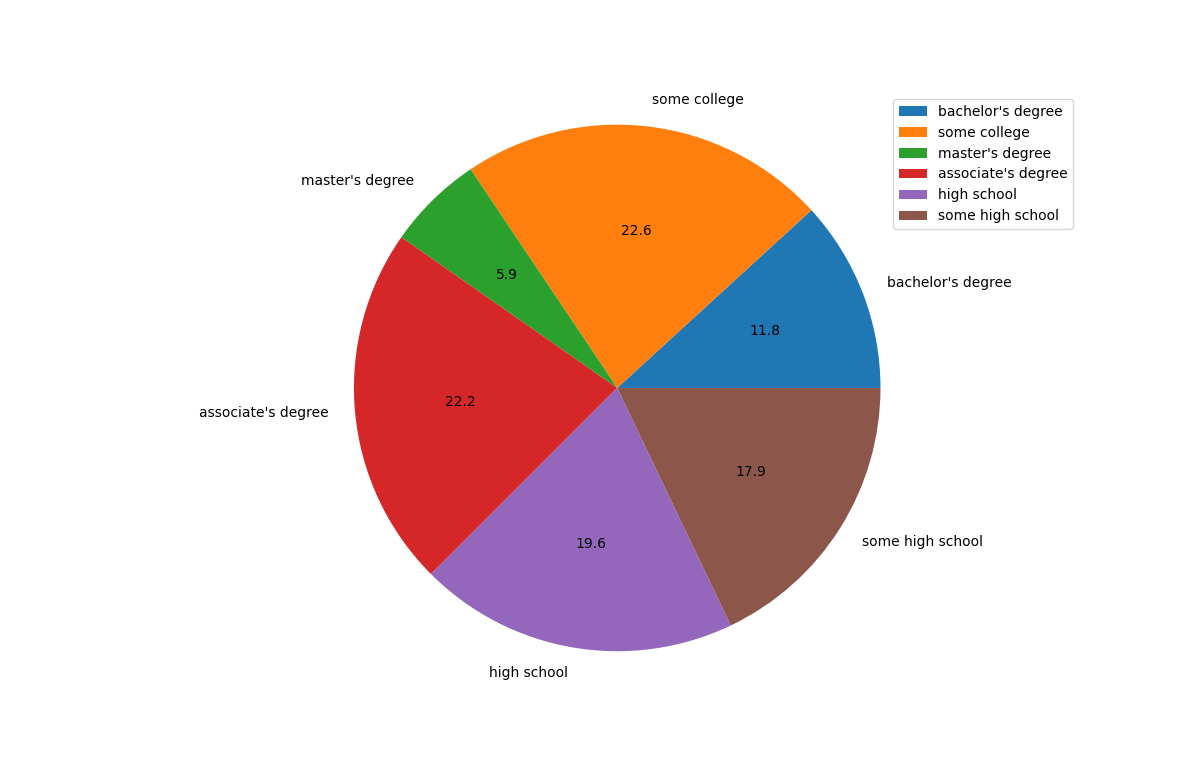
\includegraphics[scale=0.5]{parental_edu.png} 

\large \textbf{Вывод:} можно считать равным количество всех уровней образования, кроме степени магистра (master's degree). В общем и целом идёт преобладание среднего образования (колледжей, старшая школа)
\end{document}